% SANER 2027 RENE submission (RENE: NegativeResult)
% Compile with pdfLaTeX (Overleaf) or tectonic; see paper/overleaf_bundle/BUILD_README.md.
% fig1: SVG source under docs/research/figures_saner/; the bundle uses the vector PDF re-render (paper/_to_bundle_tex.py).
% Double-anonymous: the author block is intentionally anonymous for submission.
\documentclass[10pt,conference]{IEEEtran}
\usepackage{graphicx}
\usepackage{svg}
\usepackage{transparent}
\usepackage{hyperref}
\usepackage{url}
\usepackage{amsmath}
\usepackage{seqsplit}
\usepackage{array}
\hyphenation{op-tical net-works semi-conduc-tor}
\setlength{\emergencystretch}{3em}
\begin{document}
\title{Visibility Is Not Detection: Auditing Measurement Boundaries in Staged and Evidence-Ranking Evaluation}
\hypersetup{pdfauthor={},pdfsubject={},pdftitle={Visibility Is Not Detection: Auditing Measurement Boundaries in Staged and Evidence-Ranking Evaluation}}
\author{Anonymous Submission}
\maketitle
\begin{abstract}
Final-answer scores can hide the measurement boundary of a staged evaluation: a defect may be invisible to an instrument, ignored by a decision predicate, or harmless under the evaluation's equivalence contract. We audit exactly two real evaluation constructions. In Case 1, a frozen staged document evaluator, 96 of 118 controlled header injections are checkpoint-visible while the OCR-like family is unobserved on the frozen scored surface (0/13), but harmfulness remains contract-relative. In the single-responsive-leaf construction, flat and layered scores are affine/rank-equivalent, and the clean-only panel cannot identify a unique operating point. Stage-aligned instrumentation separates three constructed stages perfectly; a direct codebook does the same, while non-direct leaves retain only partial separation. FinQA is a nested boundary probe inside Case 1, not a third case. In Case 2, we audit FinRank at commit \texttt{916dc27e77b90e294ea1b3a2cc5b0abcf07392d1} under preregistered tie metrics and materiality thresholds, with one documented post-hoc identity correction after the wrong-identity v1 application. Tie policy changes absolute random-negative accuracy by about 1.03-1.08 percentage points under strict-win scoring, but changes the hard-versus-random gap by only 0.34-0.36 points and preserves its direction. The canonical \texttt{text\_sha1} identity branch reproduces 442 cross-record overlapping hard negatives across 305 records and metadata-filter gold loss in 33 records with all gold lost in 2; these are post-hoc v2 corrections. A residual reproducibility gap remains: global and metadata-filtered values drift by up to 0.19 and 0.16 points in the declared deterministic environment, while in-record and pairwise metrics reproduce exactly. The contribution is a bounded measurement audit and proposed review checklist, not a universal validity theory, detector ranking, validated universal method, or claim that either benchmark is generally defective.
\end{abstract}
\section{Introduction}
Document-intelligence systems are increasingly implemented as staged pipelines: a document is decoded, segmented into tables, mapped to a canonical schema, reconciled arithmetically, and queried. Such systems are typically scored by final-answer correctness. Final correctness, however, cannot distinguish a defect that was observed at an intermediate checkpoint from one that was silently absorbed by the pipeline, and it cannot reveal a defect that the evaluation protocol is itself unable to observe. Aggregating a pipeline into a single score therefore hides the property we care about first: whether the evaluation can observe the failures it is supposed to assess.
We keep six constructs separate throughout. \emph{Visibility} asks whether an instrument observes a change. \emph{Detection} asks whether a decision predicate consumes that observation under its threshold rule. \emph{Harmfulness} asks whether the outcome changes under a stated equivalence contract. \emph{Score sensitivity} asks how much an absolute metric moves when the scoring contract changes. \emph{Decision stability} asks whether the decision or qualitative ordering supported by the benchmark survives those changes. \emph{Reproduction gap} asks whether independently executed artifacts match the released values under a stated environment and tolerance. These six terms are audit bookkeeping for different objects, not a new causal theory or renamed reachability taxonomy. The empirical delta is that the two bounded audits separate score equivalence, contract-relative harm, score sensitivity, decision stability and reproduction failure in the same reporting surface. Confounding them makes a score gap look like protocol sensitivity, an unobserved family look like a harmful blind spot, and an absolute metric change look like a reversal of the benchmark's decision. Figure 1 shows the resulting chain from injected defect to outcome harm.
\begin{figure}[t]
\centering
% NOTE: SVG-only asset; requires the svg package + Inkscape (shell-escape) or convert to PDF/PNG
\includesvg[width=\columnwidth]{../docs/research/figures_saner/fig1_measurement_chain}
\caption{The measurement chain. An injected failure in a staged pipeline moves through checkpoint visibility (did any instrument observe it?), protocol detection (did the decision rule consume the observation under its threshold rule?), and outcome harm (does the outcome change under the stated equivalence contract?). NIST motivates measurement effectiveness, not this paper's blind-spot framework.}
\label{fig:1}
\end{figure}
This paper audits two evaluation constructions. Case 1 is a frozen staged document evaluator with controlled header perturbations and a stage-aligned instrumentation study. It exposes family-dependent visibility, affine/rank score equivalence, a non-identifiable clean calibration point and an instrumentation attribution boundary. Its FinQA program-perturbation probe is nested inside Case 1 and tests only whether the perturbation and detection predicate refer to causally aligned measurement objects. Case 2 is FinRank, a public provenance-sensitive evidence-ranking benchmark. A source-informed implementation audit examines exact tie handling, first-occurrence text/source mapping, random-negative construction and numerical reproduction. FinRank v1 tie metrics and thresholds are preregistered and unchanged; its corrected source-identity branch is explicitly post-hoc v2. The FinRank hardness ordering remains stable under alternative tie policies, while absolute pairwise values and some ranking metrics are contract-sensitive. The same case also narrows a reproducibility claim: in-record and pairwise values reproduce exactly in the audited environment, but global and metadata-filtered values do not reproduce at raw precision and the cause is unresolved.
Our contributions are:
\begin{enumerate}
\item A measurement-object separation for visibility, detection and contract-relative harmfulness in the staged evaluator, with deterministic evidence for score-structure and instrumentation identifiability.
\item A bounded FinRank evidence-ranking audit showing that tie policy and identity construction can move absolute metrics without changing the qualitative hard-versus-random decision, while keeping the post-hoc v2 identity correction and residual reproduction gap visible.
\item A proposed six-step review checklist for evaluator authors: bind mutation, observation, score, ranking and reported claim to the same measurement object; report tie and identity contracts; and state the numerical tolerance and environment required for reproducibility. This checklist is not a validated universal method.
\end{enumerate}
The accounting is intentionally narrow: there are exactly two counted cases, with FinQA nested inside Case 1. MA-CERD and adaptive revalidation are outside Paper E and contribute no case or result. The audit does not establish a universal method, a detector ranking, or a general failure rate. Its external value is narrower but concrete: it changes what should be reported and which comparisons can be interpreted before further experiments are commissioned.
\section{Related Work}
\subsection{Measurement validity and construct validity}
Meta-evaluation asks whether a metric measures what it claims. Machine-translation challenge sets such as ACES test whether a metric separates genuine errors from acceptable variants \cite{amrhein2022aces,amrhein2023aces,moghe2024mtmeta}, and contextual metric meta-evaluation extends this to local, context-dependent correctness \cite{deviyani2025contextual}. Rankings can change with protocol axes, prompt subsets, seeds, or the property a metric targets \cite{kendiukhov2026ranking,du2026stability,ross2024metric}. Reliability work on LLM-as-a-judge documents position, verbosity, self-preference, and perturbation sensitivity \cite{zheng2023judging,liq2025scoringbias,lis2025llmjduge}. Construct-validity guidance frames the same concern normatively: NIST AI 100-1 asks that TEVV metrics and processes be appropriate and effective and that measurement types be reviewed for unique and meaningful information, and NIST AI 600-1 asks that construct validity be demonstrated for each metric \cite{nist2023airmf,nist2024genai}. We share the meta-evaluation aim but ask a prior question: whether the evaluation surface can observe a controlled defect at all. We keep visibility, detection, and harmfulness as separate constructs so that a protocol comparison is not read into counts that different decision rules produce.
Recent work broadens this umbrella. Caban models validity as compounding across task generation, simulator calibration and automated judgment \cite{caban2026validity}; Bean et al. audit 445 LLM benchmarks and derive construct-validity recommendations \cite{bean2025construct}. These works already cover general validity frameworks and checklists. FinRank is closer to Case 2: it separates passage retrieval, reranking and hard-negative discrimination for provenance-sensitive financial evidence while explicitly limiting its pool to a curated passage-ranking stress test \cite{mansouri2026finrank}. Our contribution is therefore not another generic checklist. It examines whether observation surfaces, score contracts, tie order and identity construction preserve the object a concrete evaluation claims to measure.
\subsection{Testing, oracles, and diagnosability}
Mutation testing and metamorphic testing introduce controlled changes to measure whether a test or metric notices them \cite{cho2025metamorphic}; AgentChaos applies programmatic fault injection to agent systems \cite{tan2026agentchaos}. Fault-based reasoning separates whether a fault is reached, whether it changes intermediate state, and whether its effect propagates to an observable output; non-detection can arise at any of these stages, and an oracle that does not respond to a propagated effect is insensitive by construction. Process-level work evaluates intermediate behavior rather than only final success \cite{fan2026agentprocessbench,chung2026process}, and GTA-2 aggregates checkpoints recursively \cite{wang2026gta2}. We follow the mutation and fault-injection tradition but decompose non-detection into distinct mechanisms, and we treat a checkpoint forest as an evidence instrument whose diagnosability must be audited rather than assumed.
\subsection{Verified SANER RENE precedent}
The RENE track publishes reproducibility studies and negative results. Four recent papers define the surrounding practice; we describe each based on its abstract. The Limits of the Identifiable \cite{gerhold2024limits} extends deep-learning Python version identification to larger, realistic files and finds that accuracy falls from short snippets to longer segments, with import-statement analysis reaching only 30 percent, exposing limits of the approach. Does the Tool Matter? \cite{hoess2025does} compares two mining tools across ten projects and finds that even simple metrics such as commit and developer counts can differ by up to 500 percent, often from minor technical details, and hypothesizes similar uncertainty in other analysis tools. Can We Classify Flaky Tests Using Only Test Code? \cite{berndt2026flaky} evaluates three LLMs with three prompting techniques on two benchmarks and reports that classifiers are only marginally better than random, and that the test code alone does not necessarily carry enough information for a flakiness decision. Static Analysis Traces can Help Dynamic Symbolic Execution: a Replication Study \cite{kummita2026static} replicates a prior study, extends it with PhASAR-based tools and a second benchmark, and reports a conclusion different from the original: traces let KLEE find vulnerabilities about 1.4 times faster, though KLEE also confirms fewer vulnerabilities on one benchmark. These papers share our concern with measurement validity and information sufficiency; we differ in scope by auditing exactly two measurement constructions with explicit boundaries among visibility, detection, harmfulness, score sensitivity, decision stability and reproduction gap.
\section{Method}
The conceptual core is a three-way audit of visibility, detection, and harmfulness; the hierarchical checkpoint forest is the evidence instrument that makes the audit reproducible.
\subsection{Evidence instrument: checkpoint forest}
We model the pipeline as two checkpoint trees. The parsing tree covers document ingestion, table structure, field mapping, and arithmetic reconciliation. The QA tree covers retrieval grounding, faithfulness, numeric correctness, citation quality, and appropriate refusal. Together the trees contain 12 scored leaves.
The twelve scored nodes are five in the parsing tree (document status, document throughput, table regression, field hit-rate, reconciliation equations) and seven in the QA tree (retrieval contract, faithfulness judge, numeric contract, number grounding, citation judge, refusal judge, refusal contract), per the frozen checkpoint-tree configuration v0.1.0 (listed in the artifact manifest). The visibility audit exercises the parsing-tree leaves whose evidence is the mapping and regression artifacts; under the frozen drop rule (drop = (H\_orig - H\_inj) x 10, threshold 2.0) only the field hit-rate leaf responds to header drift, while QA-tree leaves keep their frozen evidence and the QA arm is reported separately (12 calls to the same judge). Additional localization value therefore remains unestablished in the current instantiation. In Table 1, the label \emph{Pruned parsing-root drop} denotes exactly this operation: the parsing root is collapsed to its single input-responsive leaf (the field hit-rate leaf) and the drop rule above is applied there.
Each leaf receives a score in [0,10]. Contractible properties use deterministic checks; semantic properties use a 0–5 judge score mapped to [0,10]. Sibling weights are normalized locally before bottom-up aggregation. Missing evidence is explicit: the parsing tree assigns 0, whereas the QA tree assigns a neutral 5. Hinge leaves affect the stability verdict, not the missing-evidence score. Every leaf stores its evidence and degradation reason.
For node n with children C(n), the recursive score is
\[
S(n)=\sum_{c\in C(n)} \frac{w(c)}{\sum_{j\in C(n)}w(j)}S(c).
\]
For a leaf, S(n) is the mapped contract or judge score. A tree is stable only when at least 90\% of its leaves exceed the selected threshold and every hinge leaf scores at least 7. The implementation is deterministic once the evidence artifacts are fixed.
\subsection{Separating visibility, detection, and harmfulness}
Visibility is defined relative to the selected checkpoint evidence surface, whereas protocol detection may use a different downstream signal.
The primary conceptual structure is the following visibility-by-detection matrix:
\begin{table}[t]
\centering
\small
\setlength{\tabcolsep}{3pt}
\begin{tabular}{>{\raggedright\arraybackslash}p{0.293\columnwidth}>{\raggedright\arraybackslash}p{0.293\columnwidth}>{\raggedright\arraybackslash}p{0.293\columnwidth}}
\hline
Checkpoint evidence & Protocol detects & Protocol does not detect \\
\hline
Visible & Detected visible defect & Visible but undetected \\
Not visible & Detection through a different signal or predicate & Silently absorbed or unobservable \\
\hline
\end{tabular}
\end{table}
Harmfulness is orthogonal to this matrix and is annotated separately as harmful, equivalent, or unresolved under the selected equivalence criterion.
For an injected defect d, visibility and protocol detection are separate observations:
\begin{itemize}
\item \textbf{Detected:} the selected protocol satisfies its detection predicate, which may test a mapping change or a score threshold.
\item \textbf{Visible but not detected:} the checkpoint exposes a difference, but the selected protocol does not satisfy its detection predicate.
\item \textbf{Silently absorbed:} normalization or matching preserves the canonical correspondence, so that the checkpoint does not expose the perturbation.
\end{itemize}
Harmfulness is a separate, \textbf{equivalence-dependent} judgment, not a mutually exclusive visibility outcome: canonical-form preservation and reader-referent recoverability need not agree.
The defect visibility profile reports visibility separately for each family. This preserves information lost by a single mutation score and distinguishes a missing checkpoint from a genuinely robust stage.
\subsection{Evaluating the evaluator}
We compare four protocols on frozen evidence: end-to-end roots, a flat leaf average, hierarchical expert weights, and hierarchical searched weights. We measure table-level detection, injection-level detection, mean separation between clean and perturbed states, worst-family behavior, localization, and evaluation cost. Because raw thresholds can manufacture differences, we separately audit (i) structural score/ranking equivalence and (ii) whether a matched-FPR operating point is identifiable from clean scores alone.
The audit further varies the injection seed, visibility threshold, matching algorithm, and scoring normalization. A semantic-judge arm is evaluated separately and never substituted for deterministic evidence when a contract exists.
\subsection{Stage-aligned instrumentation and the nested FinQA boundary probe}
The evaluation-track instrument is a two-root checkpoint forest whose twelve leaves map deterministic or judge-derived evidence to a 0–10 score (Section 3.1). To test whether stage-aligned instrumentation carries stage information, we preregister a separate controlled study on the same corpus. Each stage contract perturbs one operation: a header token is replaced (mapping stage M), required source blocks are removed from the retrieval bundle (retrieval stage R), or one numeric operand is broken while labels, schema and identity are preserved (numeric stage N). Every cluster contributes three deterministic injections, and each injection is scored on the same twelve-leaf surface, producing a binary response vector; 24 clusters per stage give 72 clusters and 216 injections. The study is frozen before results (hash receipt) and evaluated leave-one-cluster-out. The same document defines the protocol's deliberate boundary: response predicates are written from the stage contracts, so the construction is explicitly instrumented and its separability must be interpreted within that construction.
FinQA is a nested boundary probe inside Case 1, not a separate counted case. Its program-perturbation corpus acts on a step's operator or argument fields while the downstream result fields are not recomputed; the observation objects are visibility (does the injected change appear in the observed source fields), detection (does the frozen detection predicate move), and outcome (does any downstream outcome field change). The execution contract binds artifact hashes before scoring, and no threshold or convention search is permitted. Section 4.5 states the execution boundary; Section 5.6 reports what happened and what it does and does not establish.
\subsection{External evidence-ranking audit}
Case 2 is FinRank at upstream revision \texttt{916dc27e77b90e294ea1b3a2cc5b0abcf07392d1}, with arXiv record \texttt{2608.07400v1}, 1,185 released records and the official deterministic baseline implementation. The repository license is CC BY-NC 4.0. The audit follows the complete chain: question and source identity, candidate construction, scoring, global and in-record ranking, pairwise comparison, random-negative sampling, metadata filtering and published claims.
The source code exposes two known, source-informed checkpoints before application: pairwise accuracy counts exact ties for the gold (\texttt{score(gold) >= score(negative)}), and pooled-corpus passage text is deduplicated in first-occurrence order so the first occurrence supplies metadata. These probes are not presented as prospective discoveries. FinRank v1 fixed the question, tie metrics and materiality thresholds before pair-level outcomes and remains the preregistered application, but its raw-exact identity rule was wrong for FinRank's canonical contamination identity. V2 is a post-hoc deterministic correction to trimmed \texttt{text\_sha1} identity and a full reanalysis; it is not a second blind application or a wholly frozen application. The v1 tie metrics and thresholds are unchanged in v2.
The audit compares ties-positive, strict-win and half-credit pairwise policies; gold-first and negative-first ordering for exact ties inside each record; forward and reverse corpus ordering for global ranking ties; the seed-42 random-negative draw; and source-identity loss under the metadata filter. Reproducibility is checked against the released result JSON under the declared dependency versions and a second available environment. The application is deterministic and source-informed, not blind.
\section{Experimental Setup}
\subsection{Corpus and perturbations}
The study uses a frozen public tabular base and contains no client data. It includes 95 tables and 118 synthetic injections across six header-drift families. Schema and header matching are the perturbation carrier here; the object of study is the evaluation protocol's observation boundary. Each injected record preserves its source table, family, seed, changed field, and expected observation surface.
Concretely, the base is the frozen drift-v0 table set derived from public TAT-QA tables (listed in the artifact manifest by content hash); the corpus was frozen before this study's data gates and no new TAT-QA use is introduced. The perturbations are the fully synthetic injection map (listed in the artifact manifest by content hash; deterministic, seed 42, ratio 0.3). The matcher used in the audited pipeline is the greedy header matcher (listed in the artifact manifest); the cross-matcher audit adds greedy-normalized, Hungarian, and Hungarian-normalized configurations. Semantic leaves are scored by the judge pipeline (listed in the artifact manifest), i.e. Qwen3.6-35B-A3B (Q4\_K\_M GGUF) served locally, with 0–5 dimension scores mapped to [0,10]. The primary threshold grid is
\[
\Gamma=\{0.2,0.3,0.5,0.7,0.9\}.
\]
The OCR-like family contains 13 single-token, lowercase Levenshtein-distance-one substitutions with unchanged column values. These properties are mechanically recomputed before interpretation.
\subsection{Baselines and controls}
The protocol baselines are end-to-end scoring, flat leaf scoring, and hierarchical scoring with expert weights. Weight-search controls include equal weights, expert weights, 30 random trials, greedy coordinate ascent, particle-swarm optimization (PSO), and a minimax objective. Assignment controls compare greedy matching with Hungarian global assignment and include a positive solver test.
\subsection{Statistical discipline}
We freeze inputs and decision criteria before reading each result. Confidence intervals are reported on table-level clustered units where available (percentile bootstrap over the 95 table units, seed 20260830; endpoints on the k/95 grid for the 95-table arm). Seed sensitivity uses three injection seeds. For the clean-only matched-FPR audit, threshold selection may use clean scores only; injected and harmful outcomes are prohibited from calibration. Because the frozen clean supports are degenerate, the registered deployment operating point is left unresolved rather than forced into an empirical equality. The 2,382 clean records are the usable (table\_uid, column) rows of the non-injected source tables in the frozen clean-input set, with fold assignment = sorted(table UID) index modulo 5. Null and adverse findings are retained rather than relabeled as improvements.
\subsection{Multi-leaf stage-aligned protocol}
The stage-aligned study uses the same frozen tabular base and the same twelve-leaf surface. Stage contracts and injection generators are deterministic; clusters are selected by an outcome-blind hash rule (seed frozen before results), and the pre-result freeze receipt binds the corpus, the generator, the runner and the environment by hash. Response predicates are contract-derived: for M the directly targeted parse leaves move; for R the retrieval leaf moves; for N the reconciliation leaf moves. Baselines are the metric-specific chance top-1 (1/3) and majority macro-F1 (1/6); uncertainty uses leave-one-cluster-out evaluation with 10,000 cluster-bootstrap resamples and a 10,000-replicate permutation null, both seeds frozen. The ablation re-scores the same rows with (i) the full twelve-leaf vector, (ii) the fixed three-direct-leaf codebook, (iii) non-direct leaves only, and (iv) a single any-response scalar.
\subsection{Second-dataflow execution boundary}
The nested FinQA boundary probe executes a frozen step-perturbation corpus under a hash-bound binding contract: 89 rows over 30 clusters, with per-row runtime bindings and a full trace map verified before scoring. The perturbation writes operator/argument fields; the observation vector records visibility, detection and outcome per row. Because downstream result fields are not recomputed from the mutated program semantics by construction, a zero detection count in this execution is not an estimate of detection ability; Section 5.6 states the resulting measurement-object boundary and the alternatives the evidence does not exclude. No threshold search, convention selection, or source-operator substitution is permitted in this probe. It is nested inside Case 1 and does not increase the case count.
\subsection{FinRank external audit setup}
FinRank contains manually authored questions, reference answers, gold passages and curated hard negatives over 22 companies. The released global pool contains 5,230 unique raw passage texts. The audit uses only the released JSONL, repository code, split/random seed and result files. TF-IDF and BM25 are regenerated from the official script with its released parameters; neural baselines are outside this audit.
The primary proposition was fixed before pair-level outcomes: the tie-positive policy and first-occurrence identity mapping may change absolute metric interpretation, while the paper's narrow curated-pool contract may keep the hard-versus-random conclusion stable. V1 materiality thresholds are 1.0 percentage point for pairwise values or hardness-gap movement and 0.5 point for global tie-order movement, and they remain unchanged after the post-hoc v2 identity correction. The outcome classes are interpretation changed, narrower contract stable, or no substantive impact.
\section{Results}
\subsection{Visibility depends on defect family}
Checkpoint-level analysis makes 96/118 injections visible, but the aggregate hides a large family effect. 0/13 OCR-like injections were visible across 11 table clusters under all five thresholds; all 13 were invisible under this observation criterion. Other families range from 0.81 to 1.00 visibility at the primary setting. For uncertainty, the injection-level reference estimand is 0/13 with an exact binomial 95\% interval of [0, 24.71\%] under an independent-injection assumption; the distinct table-level event estimand is 0/11 with an exact binomial interval of [0, 28.49\%]. The latter is not a clustered confidence interval for injection-level visibility. Figure 2 reports the full family-by-threshold visibility profile.
\begin{figure}[t]
\centering
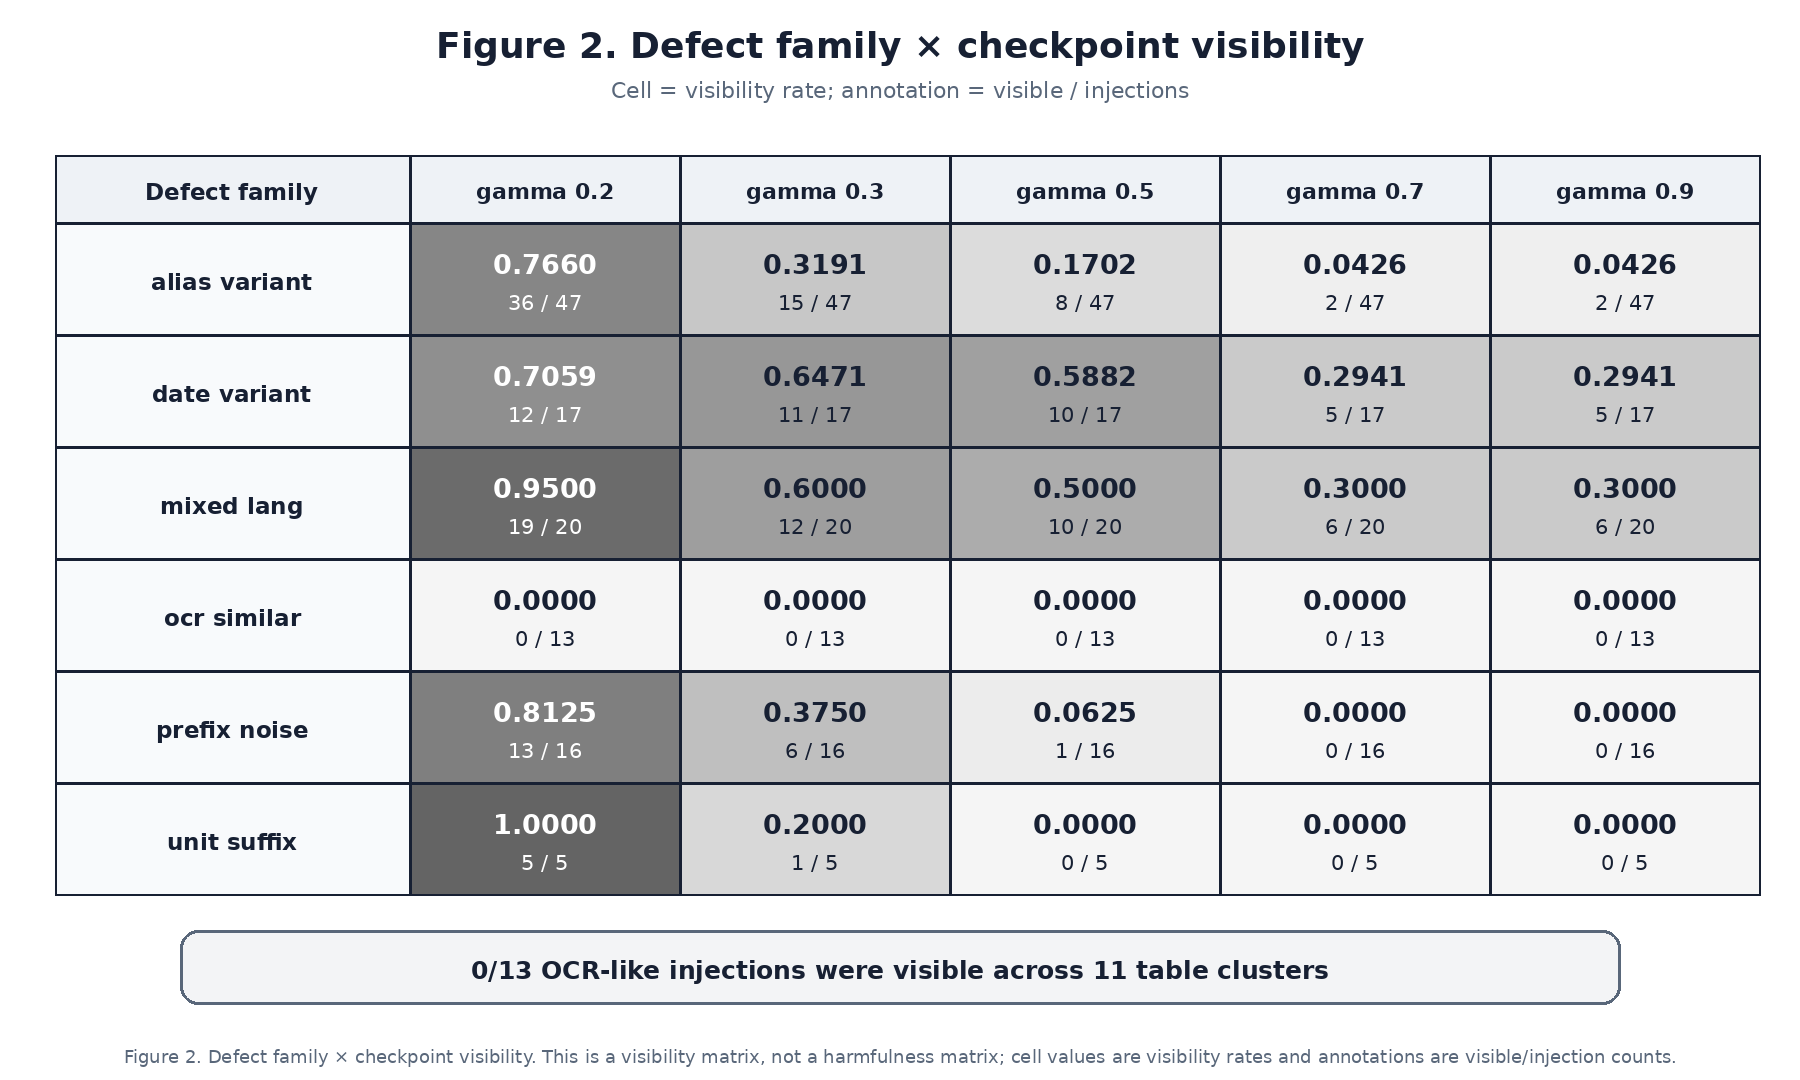
\includegraphics[width=\columnwidth]{../docs/research/figures_saner/fig2_family_visibility_matrix.png}
\caption{Defect family × checkpoint visibility. Cell values are visibility rates at each threshold, annotated with visible/injection counts; the OCR-like family is 0/13 across 11 clusters at every tested threshold. This is a visibility matrix, not a harmfulness matrix.}
\label{fig:2}
\end{figure}
The family unobserved on the frozen scored surface remains the same under four edit-distance matcher configurations. However, the ordering of visible families is not invariant: changing the score normalization causes five class flips, all within the date-variation family, whereas switching from greedy to global assignment causes no flips. Thus, the existence of a family unobserved on the frozen scored surface is stable within the tested matcher family, but the full ranking is protocol-dependent.
The harmfulness label is also criterion-dependent, and our record contains two comparison kinds that should not be pooled. In the first kind, seven paired judge-versus-standard comparisons yield four disagreements; the two standards differ in the criterion they apply, with the standard asking whether the canonical form and canonical truth survive and the judge asking whether a reader can recover the same referent. In the second kind, a single visibility-versus-equivalence comparison contrasts deterministic channel evidence with standard equivalence, and that case carries no judge call. Because the two kinds measure different objects, we keep the raw cases and report neither a pooled disagreement rate nor a mechanism that would exclude case-level noise. In particular, the existing single judge, applying its table-context reader-referent contract, classified all 13 OCR-like perturbations as referentially equivalent. That supports benign absorption as an alternative interpretation of the non-response; it is not independent ground truth, and non-response alone does not establish harmful false negatives. We therefore report that this family is unobserved on the frozen scored surface, while treating whether that absence is harmful as a boundary question.
\subsection{The raw hierarchy gap is a threshold-placement artifact}
The raw detection counts are not evidence of protocol discriminability. Table 1 compares three transferable protocols under different decision predicates: end-to-end detection tests whether the final mapping text changes, whereas flat and hierarchical scoring use frozen score-drop thresholds. A changed source-header string can therefore count as end-to-end detection even when the canonical match is preserved, explaining why 112/118 exceeds the 96/118 visibility count. Table-level counts apply all assigned injections together, whereas injection-level counts apply one perturbation at a time; the 20 detected tables and 13 individually detected injections are not nested counts. At the frozen threshold, hierarchical scoring is not a more sensitive detector.
\textbf{Table 1. Protocol-level detection under different decision predicates.}
\begin{table}[t]
\centering
\small
\setlength{\tabcolsep}{3pt}
\begin{tabular}{>{\raggedright\arraybackslash}p{0.220\columnwidth}>{\raggedright\arraybackslash}p{0.220\columnwidth}>{\raggedright\arraybackslash}p{0.220\columnwidth}>{\raggedright\arraybackslash}p{0.220\columnwidth}}
\hline
Protocol & Detection signal & Tables detected & Injections detected \\
\hline
End-to-end & Final mapping change & 95/95 (1.0000) & 112/118 (0.9492) \\
Flat & Field-hit-rate drop & 75/95 (0.7895; 95\% CI [0.6947, 0.8737]) & 85/118 (0.7203) \\
Hierarchical, expert weights & Pruned parsing-root drop & 20/95 (0.2105; 95\% CI [0.1263, 0.2947]) & 13/118 (0.1102) \\
\hline
\end{tabular}
\end{table}
The raw flat-hierarchical gap does not establish inferior ranking quality. In the current single-responsive-leaf construction, the unrounded hierarchical contrastive score is a positive rescaling of the flat contrastive score, with fitted slope approximately 0.375, and the recorded scores retain identical ranks; corresponding decisions, and by implication their ROC geometry, therefore coincide, and corresponding thresholds satisfy theta\_H = 0.375 theta\_F. This is a structural equivalence of the two protocols' decisions, not a newly calibrated performance estimate; the diagnosis is deliberately narrow: it explains why the raw protocol gap cannot be read as a ranking difference, and it is not offered as a general algebraic result about hierarchical evaluation. Separately, the registered deployment operating point remains unresolved: the derived clean-only reanalysis contains 2,382 usable clean records whose score supports are exactly \{0\}, so every positive threshold has an observed FPR of zero and the clean panel cannot select a unique operating point. That calibration degeneracy does not negate the structural equivalence, and it is a statement about the current clean-only procedure, not a general claim that matched-FPR comparisons cannot be made; the registered strict predicate FPR = alpha and the tolerance predicate FPR <= alpha also remain distinct. Selecting a threshold by harmful TPR would violate the clean-only contract. Historical fixed-threshold sensitivity evidence remains in the dated historical governance record, but the old [0,0] interval is not a clean-calibrated confirmatory result. When more than one leaf varies with the input, neither affine nor ranking equivalence is guaranteed.
The 118 injections close at the checkpoint level as 96 visible plus 22 silently absorbed; by family (injections / visible / absorbed): alias variant 47/43/4, date variant 17/15/2, mixed language 20/20/0, OCR-like 13/0/13, prefix noise 16/13/3, unit suffix 5/5/0 (frozen artifact listed in the evidence ledger). The protocol-level counts in Table 1 are measured on different signals and are therefore not a partition of the 96.
We label the affine-equivalence observation a degenerate-case result: it fixes the interpretation of the raw gap under the current single-varying-leaf construction and does not establish affine equivalence of the protocols in general.
\subsection{Sensitivity and reproducibility}
The identity of the family unobserved on the frozen scored surface is stable across the threshold grid. The absolute between-family range shrinks at high thresholds, as expected when one changed header contributes at most 1/n for a table with n canonical headers. The literal preregistered range criterion fails at 0.7 and 0.9, and this failure is reported.
Across three injection seeds, flat table-detection rates are 75/95 = 0.7895, 76/97 = 0.7835, and 68/90 = 0.7556. Their spread is 0.0339; the denominator-weighted pooled rate is 219/282 = 0.7766 with a percentile bootstrap 95\% interval of [0.7270, 0.8227] over the pooled 282 table units (seed 20260830; endpoints on the k/282 grid). The seed-42 run reproduces the frozen artifact byte-for-byte.
Judge calibration covers 120 leaf-state cells; this calibration window is distinct from the 28-case semantic boundary analysis reported in Section 6. In the control-state comparison, rejudged summaries of historical 0–5 judgments differ from the frozen dimension means by at most 0.5, meeting the preregistered consistency expectation. This checks reproduction of aggregate dimension scores, not agreement between judges re-evaluating the same original answers. On the derived 0–10 root scale, control roots differ by at most 0.22, while individual leaves can move by as much as 7.0. Agreement is therefore an aggregate observation, not evidence of cell-level interchangeability.
\subsection{Weight search produces an informative null}
PSO and greedy coordinate ascent reach the same mean separation of 1.432574. PSO repeats the result on all five seeds but requires 7,650 evaluations, compared with 67 for greedy search. A minimax variant improves worst-case separation to 0.35714 while reducing mean separation to 1.25605. We therefore do not claim PSO superiority. The result instead shows that objective choice matters more than optimizer sophistication in the present search space.
\subsection{Stage-aligned instrumentation: separable signatures and their boundary}
\begin{figure}[t]
\centering
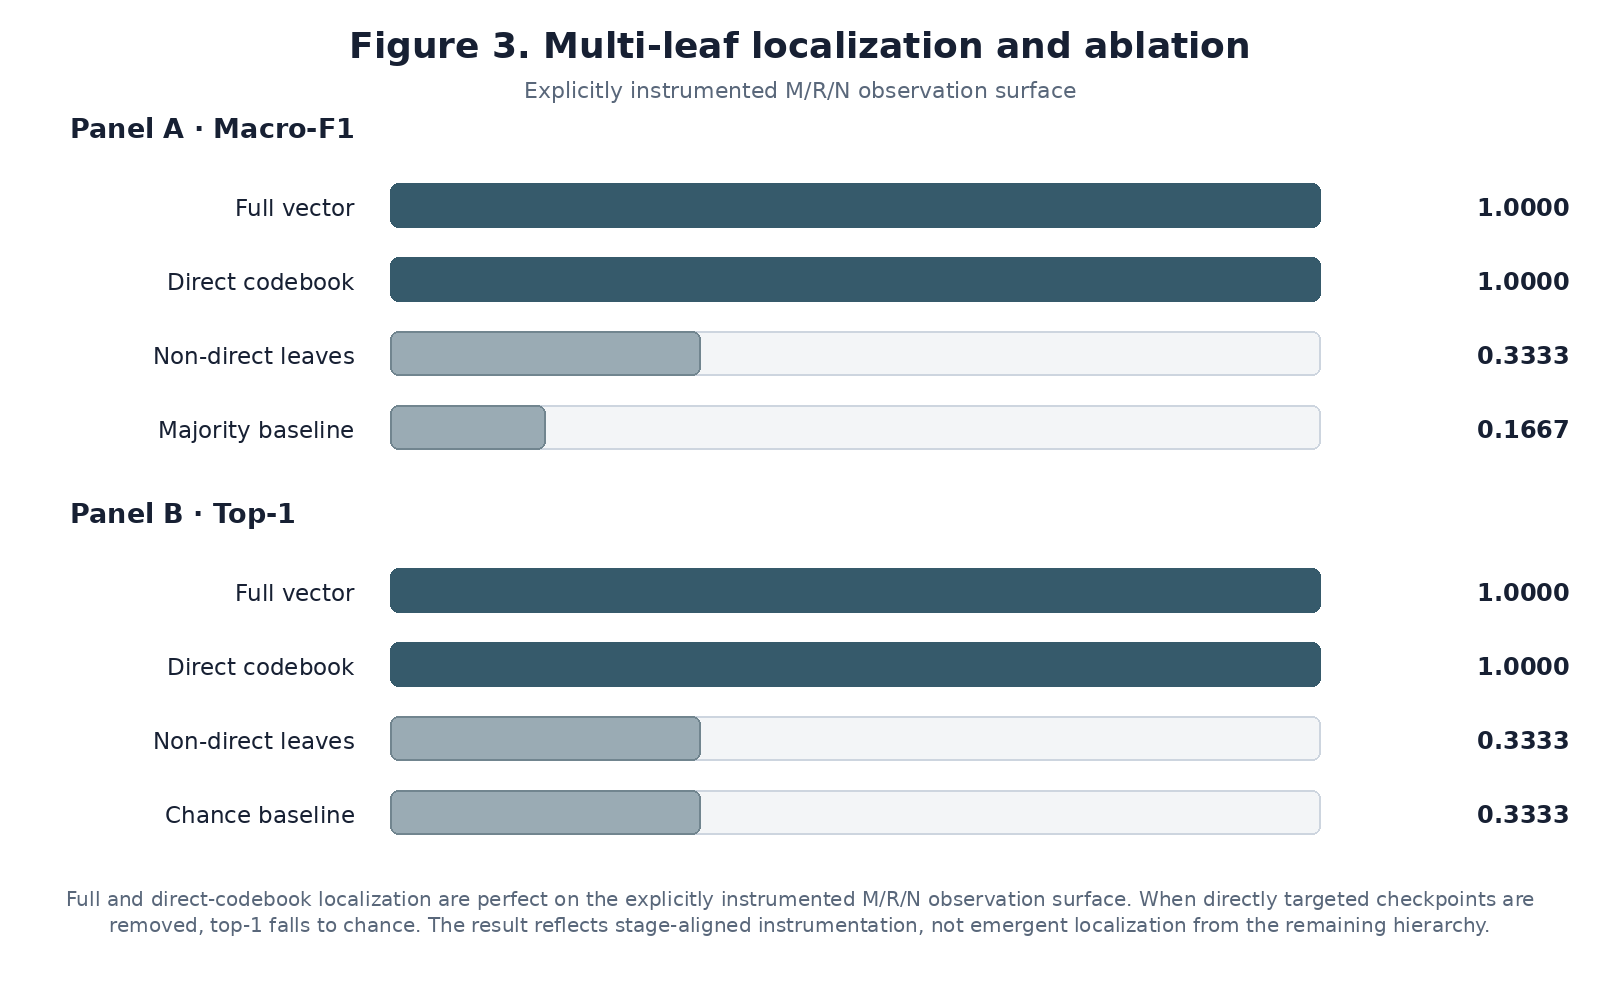
\includegraphics[width=\columnwidth]{../docs/research/figures_saner/fig3_localization_ablation.png}
\caption{Multi-leaf localization and ablation. Perfect full-vector and direct-codebook bars are construct-sensitive on the explicitly instrumented controlled M/R/N observation surface. After directly targeted checkpoints are removed, non-direct top-1 equals chance (0.3333); under the frozen tie-as-incorrect rule these leaves still separate mapping from the retrieval and numeric stages without separating retrieval from numeric. Non-direct macro-F1 equals the uniform-class macro-F1 baseline (0.3333); the majority-class macro-F1 reference (0.1667) is plotted. The result reflects stage-aligned instrumentation, not emergent localization from the remaining hierarchy.}
\label{fig:3}
\end{figure}
The preregistered stage-aligned study separated the three controlled stages perfectly on the explicitly instrumented surface: leave-one-cluster-out macro-F1 and top-1 accuracy are 1.000 with cluster-bootstrap 95\% intervals [1.0, 1.0] and permutation p = 1/10001 = 1e-4, with zero ties and zero errors, against metric-specific baselines (chance top-1 1/3; majority macro-F1 1/6). The per-stage response profiles are disjoint within the construction: M moves the field-hit and table-regression leaves, R moves the source-required leaf, and N moves the reconciliation leaf. Figure 3 reports the localization and ablation outcome.
That positive result carries its boundary in the same rows. Re-scoring the identical 216 injections with the fixed three-direct-leaf codebook also yields macro-F1 and top-1 of 1.000; the non-direct leaves alone fall to 0.3333 with a tie rate of 0.6667, which is the three-class chance level and the uniform-class macro-F1 baseline; under the frozen tie-as-incorrect rule they distinguish the mapping stage from the retrieval and numeric stages but do not distinguish retrieval from numeric, so they carry partial rather than no stage information. A single any-response scalar collapses to 0.0 with ties everywhere. Eight of the twelve leaf columns are identically zero over all injections. Perfect separability therefore reflects explicit stage-aligned instrumentation in a contract-derived construction, not emergent localization from the remaining hierarchy, and the positive result is reported together with this ablation. Per-stage estimates are descriptive at this sample size; the population is the frozen controlled injection set, not a natural-failure distribution.
\subsection{Nested Case 1 boundary probe: measurement-object mismatch}
The nested FinQA probe produced V = 89/89, D = 0/89 and O = 0/89: every injected change was observable on the mutated source fields, the frozen detection predicate never moved, and no downstream outcome field changed. The detection predicate here is defined and executable, and these counts are reproducible; what the perturbation does not do is regenerate the downstream result fields that the predicate reads. The zero detection count therefore describes this carrier construction rather than an estimated detection ability, and the mismatch is one of measurement objects, not of predicate definition. The formal result class is a mixed second-flow outcome; the accepted interpretation is a measurement-object mismatch, recorded in a separate autopsy. This is a boundary probe inside Case 1, not a third case. We therefore treat causal alignment of measurement objects as a design requirement for future transfers, not as a validated law. Scorer non-portability, threshold non-transfer and corpus shift are not excluded by this evidence, and no transfer, blindness or semantic-correctness claim is made from this probe.
\subsection{Case 2: stable hardness decision, sensitive score contract}
The compact FinRank result separates score sensitivity from decision stability. Values are hard/random pairwise accuracy and the random-minus-hard gap in percentage points:
\begin{table}[t]
\centering
\small
\setlength{\tabcolsep}{3pt}
\begin{tabular}{>{\raggedright\arraybackslash}p{0.176\columnwidth}>{\raggedright\arraybackslash}p{0.176\columnwidth}>{\raggedright\arraybackslash}p{0.176\columnwidth}>{\raggedright\arraybackslash}p{0.176\columnwidth}>{\raggedright\arraybackslash}p{0.176\columnwidth}}
\hline
Model & Tie policy & Hard & Random & Gap \\
\hline
TF-IDF & ties-positive & 77.756 & 91.935 & 14.179 \\
TF-IDF & strict-win & 77.030 & 90.850 & 13.821 \\
TF-IDF & half-credit & 77.393 & 91.393 & 14.000 \\
BM25 & ties-positive & 74.780 & 87.789 & 13.009 \\
BM25 & strict-win & 74.094 & 86.760 & 12.666 \\
BM25 & half-credit & 74.437 & 87.275 & 12.838 \\
\hline
\end{tabular}
\end{table}
Exact ties occur in both deterministic score matrices. TF-IDF has 91 hard-pair and 135 random-pair ties; BM25 has 83 and 125. Changing ties-positive to strict-win moves random-negative accuracy by 1.084 points for TF-IDF and 1.029 for BM25, crossing the preregistered 1.0-point materiality threshold. This is score sensitivity. By contrast, the hard-versus-random gap moves by only 0.358 and 0.343 points and retains its direction under strict-win and half-credit scoring. This is decision stability for the narrow qualitative hardness claim. Five of 11,790 seed-42 random draws equal a curated hard negative, too few to explain the gap.
Tie order is a separate sensitivity probe. Inside each record, concatenating gold before negatives makes exact ties gold-first. Reversing tie priority lowers MRR by 0.101-0.108 points and nDCG@5 by 0.572-0.573 points. Forward-versus-reverse corpus order changes top-level global ranking metrics by at most 0.287 point, below the preregistered 0.5-point threshold. Absolute scores and small ranking differences are therefore contract-sensitive, while the qualitative ordering remains stable under the tested alternatives.
The identity audit is explicitly post-hoc v2 after the wrong-identity v1 application. These are corrections to this audit's identity implementation, not corrections to FinRank itself. The canonical \texttt{text\_sha1} branch reproduces the source-informed, author-disclosed target quantities of 442 hard-negative occurrences across 305 records sharing a canonical text identity with another record's gold. Raw exact matching's 293/220 result is the superseded v1 identity rule. First-occurrence metadata filtering reproduces the known source-informed counts of gold loss in 33 records and all-gold loss in 2. The counts are deterministic post-hoc reproductions, not preregistered observations from a wholly frozen application.
Reproduction remains a separate construct. In-record MRR/nDCG and all pairwise metrics reproduce exactly. Top-level global ranking metrics differ from the bundled result JSON by up to 0.19 point and metadata-filtered metrics by up to 0.16 point in the declared deterministic environment; a second available environment changes some global values by as much as 0.47 point, while slice aggregates drift by as much as 0.51 point. Without the original score matrices or complete execution environment, the residual global and metadata metric drift cannot be attributed uniquely to tie order or dependency drift. Its cause is unresolved, and the result is a reproducibility boundary rather than a benchmark failure.
\section{Discussion and Limitations}
The two counted cases support one measurement discipline without collapsing its constructs. Visibility, detection and harmfulness concern instruments, predicates and equivalence contracts. Score sensitivity, decision stability and reproduction gap concern absolute metrics, the decision a benchmark supports and the execution envelope. FinRank makes the latter three separation concrete: tie policy materially changes absolute pairwise scores, the qualitative hard-versus-random decision remains stable under tested alternatives, and residual global or metadata metric drift remains unexplained.
\subsection{Scientific limitations}
The staged case remains narrow. It uses synthetic perturbations on one public tabular corpus; no natural-failure distribution or cross-domain generalization is measured. Harmfulness is equivalence-dependent. The OCR-like family is unobserved on the frozen scored surface rather than proven harmful, and the existing single judge classified all 13 cases as referentially equivalent under its table-context contract. The semantic boundary analysis uses one judge on 28 cases; mixed-language and unit-suffix families receive no calls in that window, which is separate from the 120-cell judge calibration of Section 5.3. Under shared-header overlays the oracle correctness ceiling changes from 20/21 = 0.952381 to 40/67 = 0.597015 using different denominators, while global assignment changes no decision. Perfect stage localization is explained by explicit stage-aligned instrumentation. The nested FinQA probe fails because its perturbed program does not regenerate the result fields read by the detector; this is a measurement-object boundary, not evidence of protocol blindness.
The FinRank case is similarly bounded. V1 fixed the question, tie metrics and materiality thresholds before pair-level outcomes, but used the wrong source-identity rule. The canonical \texttt{text\_sha1} counts of 442/305 and 33/2 are post-hoc v2 corrections after that wrong-identity application. V2 preserves the v1 tie values and thresholds but is a post-hoc corrected implementation, not a wholly frozen application. The audit covers TF-IDF and BM25, not neural baselines, and does not evaluate answer generation. It is source-informed because the paper and code disclose tie and identity behavior before application. The exact cause of residual global and metadata metric drift is unresolved without the original score matrices or a locked transitive environment.
MA-CERD and adaptive revalidation are not Paper E cases and provide no evidence here. The later AI-assisted 24-task review and deferred model-free or scoring routes are internal-only historical development records, not submission results. They are excluded from the counted cases, contribution and reported findings.
\subsection{Proposed six-step review checklist}
The following sequence is a proposed checklist for evaluator authors, not a validated universal method:
\begin{enumerate}
\item identify the observation surface and its instruments;
\item bind each perturbation to the recomputed measurement object;
\item inspect score algebra, tie policy and threshold identifiability;
\item preserve source identity and equivalence contracts;
\item test whether the result changes a real report, model-selection or measurement decision;
\item report negative or stable results and the exact reproducibility envelope.
\end{enumerate}
\subsection{Integrated interpretation}
Case 1 removes three tempting over-readings: a visible score gap is not automatically a performance gap; an unobserved family is not automatically a harmful blind spot; and separability does not follow from hierarchical organization when the response predicates are explicitly stage-aligned. Its FinQA probe adds a measurement-object requirement without becoming a third case. Case 2 separates score sensitivity from decision stability and exposes a reproduction gap whose cause is unresolved. Together they show why mutation, observation, score, ranking and reported claim must be bound to the same causally updated measurement object before a cross-system comparison is interpreted. The evidence remains limited to exactly these two cases.
\section{Conclusion}
Final correctness or aggregate ranking quality does not reveal whether a staged evaluation observed a defect, consumed an intermediate signal, preserved source identity, or reproduced its released values. Across exactly two cases, a controlled staged document evaluator and the FinRank evidence-ranking audit, we keep visibility, detection, harmfulness, score sensitivity, decision stability and reproduction gap separate. In Case 1, family-level visibility, score equivalence, instrumentation attribution and the nested FinQA measurement-object boundary remove several tempting over-readings. In Case 2, tie policy moves absolute pairwise scores while the qualitative hard-versus-random decision remains stable; the 442/305 and 33/2 identity counts are post-hoc v2 corrections after the wrong-identity v1 application; and residual global and metadata metric drift remains unexplained. The result is a bounded two-case measurement audit and a proposed checklist, not a universal validity theory, validated universal method or detector ranking.
\section{Data Availability}
The staged evaluation corpus is derived from public TAT-QA tables. Frozen perturbation, checkpoint, aggregation and analysis artifacts, together with exact revisions and hashes, are prepared as an anonymized release package. The nested FinQA probe is described by its frozen activation record; it is a Case 1 boundary probe, not a counted case. Case 2 uses FinRank revision \texttt{916dc27e77b90e294ea1b3a2cc5b0abcf07392d1}, arXiv \texttt{2608.07400v1}, the released \texttt{FinRank.jsonl}, baseline code and result JSON under CC BY-NC 4.0.
The preregistered wrong-identity v1 application is preserved unchanged. The canonical \texttt{text\_sha1} 442/305 and 33/2 identity results are labelled post-hoc v2 corrections; no raw score or 2026-10-21 correction/recomputation evidence is overwritten. The residual global and metadata reproduction gap is disclosed with its cause unresolved. The audit script, preregistration, fixtures, full application rows and source manifest are included in the preserved evidence package. No private data, model inference or paid research API is required to reproduce the deterministic audit. The AI-assisted 24-task review and deferred model-free/scoring routes remain internal-only historical records outside the submission package. An anonymized repository and persistent DOI are not yet established.
\bibliographystyle{IEEEtran}
\bibliography{saner_rene_references}
\end{document}
